\documentclass[aspectratio=169]{beamer}
\usepackage{dbt}

%%%% Standard packages
\usepackage{graphicx}
\usepackage{epstopdf}
\usepackage{multirow}
\usepackage{cancel}
\usepackage{bm} % bold math
\usepackage[squaren,thickqspace]{SIunits}
% \usepackage{animate}
% Packages for typesetting algorithms and good looking pseudocode 
\usepackage{algorithm}
\resetcounteronoverlays{algorithm}
\usepackage[noend]{algpseudocode}
% Handling tables
\usepackage{booktabs}
\usepackage[boldmath]{numprint}
\usepackage{wrapfig}

%%%% TIKZ
\usepackage{tikz}
\usepackage{caption}
\usetikzlibrary{decorations.pathreplacing,shapes,arrows,positioning}
\tikzset{
	vertex/.style = {
		circle,
		fill            = black,
		outer sep = 2pt,
		inner sep = 1pt,
	}
}
\usetikzlibrary{spy}
\usetikzlibrary{matrix}
\usetikzlibrary{overlay-beamer-styles}

% Handling units
\usepackage[squaren,thickqspace]{SIunits}
\addunit{\pixel}{pixel}
\addunit{\pixels}{pixels}
\addunit{\voxel}{voxel}
\addunit{\decibel}{dB}
\addunit{\byte}{B}
\addunit{\hounsfield}{HU}

% Handling tables
\usepackage{booktabs}
\usepackage[boldmath]{numprint}

\setbeamercolor{emph}{fg=hilight}
\renewcommand<>{\emph}[1]{%
	{\usebeamercolor[fg]{emph}\only#2{\itshape}#1}%
}

\setbeamercolor{alert}{fg=vhilight}
\renewcommand<>{\alert}[1]{%
	{\usebeamercolor[fg]{alert}\only#2{\itshape}#1}%
}

\setbeamercolor{section in head/foot}{fg=title}
\setbeamertemplate{footline}
{
	\leavevmode%
	\hbox{%
		\begin{beamercolorbox}[wd=.333333\paperwidth,ht=2.25ex,dp=1ex,center]{section in head/foot}%
			\usebeamerfont{author in head/foot}\insertshortauthor
		\end{beamercolorbox}%
		\begin{beamercolorbox}[wd=.333333\paperwidth,ht=2.25ex,dp=1ex,center]{section in head/foot}%
			\usebeamerfont{title in head/foot}\insertshorttitle
		\end{beamercolorbox}%
		\begin{beamercolorbox}[wd=.333333\paperwidth,ht=2.25ex,dp=1ex,right]{section in head/foot}%
			\usebeamerfont{date in head/foot}\insertshortdate{}\hspace*{2em}
			\insertframenumber{} / \inserttotalframenumber\hspace*{2ex} 
		\end{beamercolorbox}}%
		\vskip0pt%
	}
	\makeatother

% Semi-visible itemize
\setbeamercovered{invisible}
\setbeamercovered{%
	again covered={\opaqueness<1->{60}}}

% Place logos in the title page
\titlegraphic{%
	\begin{minipage}{0.33\textwidth}
		\centering
		\includegraphics[height=50pt]{KTH_Logotype}
	\end{minipage}%
	\begin{minipage}{0.33\textwidth}
		\centering
		\includegraphics[height=50pt]{Elekta-vertical.pdf}
	\end{minipage}%
	\begin{minipage}{0.33\textwidth}
		\centering
		\includegraphics[height=50pt]{SSF_Logotype.png}
	\end{minipage}%
}
% backup slides
\newcommand{\backupbegin}{
	\newcounter{framenumberappendix}
	\setcounter{framenumberappendix}{\value{framenumber}}
}
\newcommand{\backupend}{
	\addtocounter{framenumberappendix}{-\value{framenumber}}
	\addtocounter{framenumber}{\value{framenumberappendix}} 
}

% Declare image layers
% By default all math in TikZ nodes are set in inline mode. Change this to
% displaystyle so that we don't get small fractions.
\everymath{\displaystyle}

%%%% Macros 
% Sets
\newcommand{\Real}{\ensuremath{\mathbb{R}}}
\newcommand{\Complex}{\ensuremath{\mathbb{C}}}
\newcommand{\Integer}{\ensuremath{\mathbb{Z}}}
\newcommand{\Natural}{\ensuremath{\mathbb{N}}}
\newcommand{\domain}{\Omega}
\newcommand\datamanifold{\mathbb{M}}
\newcommand\trainingdata{\mathcal{M}}
% Spaces
\newcommand{\RecSpace}{\ensuremath{X}}
\newcommand{\DataSpace}{\ensuremath{Y}}
\newcommand{\ParamSpace}{\ensuremath{Z}}
\newcommand{\ProdSpace}{\ensuremath{U}}
\newcommand{\FeatureSpace}{\ensuremath{\mathbb{F}}}
% Operators
\newcommand{\approxInv}[1]{#1^{\dagger}}
\newcommand{\learnedInv}[1]{#1^{\dagger}}
\DeclareMathOperator{\IdentityOp}{\ensuremath{\text{Id}}}
\DeclareMathOperator{\OpA}{\ensuremath{\mathcal{A}}}
\DeclareMathOperator{\OpB}{\ensuremath{\mathcal{B}}}
\DeclareMathOperator{\OpC}{\ensuremath{\mathcal{C}}}
\DeclareMathOperator{\OpF}{\ensuremath{\mathcal{F}}}
\DeclareMathOperator{\OpG}{\ensuremath{\mathcal{G}}}
\DeclareMathOperator{\OpK}{\ensuremath{\mathcal{K}}}
\DeclareMathOperator{\ForwardOp}{\ensuremath{\mathcal{T}}}
\DeclareMathOperator{\ForwardOpPseudoInv}{\ensuremath{\approxInv{\ForwardOp}}}
\DeclareMathOperator{\ForwardOpInvLearned}{\ensuremath{\learnedInv{\ForwardOp}_{\param}}}
\DeclareMathOperator{\RadonTransform}{\ensuremath{\mathcal{P}}}
\DeclareMathOperator{\LogLikelihood}{\ensuremath{\mathcal{L}}}
\DeclareMathOperator{\AffineOp}{\ensuremath{\mathcal{W}}}
\DeclareMathOperator{\NonLinOp}{\ensuremath{\OpA}}
\DeclareMathOperator*{\argmin}{arg\,min}
\DeclareMathOperator{\errorfunc}{E}
\DeclareMathOperator{\RegOp}{\mathcal{S}}
\DeclareMathOperator{\DataDiscr}{\mathcal{D}}
\DeclareMathOperator{\loss}{L}
\DeclareMathOperator{\objective}{\mathcal{E}}
\DeclareMathOperator{\distance}{d}
\DeclareMathOperator{\Id}{Id}
\DeclareMathOperator{\grad}{\nabla\!}
\DeclareMathOperator{\ProxOp}{\ensuremath{prox}}
\DeclareMathOperator{\esssup}{\ensuremath{ess\,sup}}
\DeclareMathOperator{\FeatureExt}{\ensuremath{\mathcal{R}}}
% Probabilistic concepts
\newcommand{\stochastic}[1]{\mathsf{#1}}
\newcommand{\stsignal}{\stochastic{\signal}}
\newcommand{\stdata}{\stochastic{\data}}
\DeclareMathOperator{\ProbdistFunctional}{\stochastic{F}}
\DeclareMathOperator{\Expect}{\mathbb{E}}
\DeclareMathOperator{\Variance}{Var}
\newcommand{\ProbabilityDistribution}{\stochastic{P}}
\newcommand{\ProbabilityMeasure}{\mu}
% Elements in spaces
\newcommand{\signal}{\ensuremath{f}}
\newcommand{\signalother}{\ensuremath{h}}
\newcommand{\signaltrue}{\signal_{\text{true}}}
\newcommand{\mollifier}{\ensuremath{e}}
\newcommand{\data}{\ensuremath{g}}
\newcommand{\noise}{\delta\data}
\newcommand{\signallearned}[1]{\ForwardOpInvLearned(#1)}
\newcommand{\memory}{s}
\newcommand{\param}{\ensuremath{\theta}}
\newcommand{\weight}{\ensuremath{w}}
\newcommand{\vweight}{\ensuremath{\boldsymbol{\weight}}}
\newcommand{\bias}{\ensuremath{b}}
\newcommand{\primal}{\ensuremath{f}}
\newcommand{\dual}{\ensuremath{h}}

\newcommand{\altemph}[2]{\alt<#1>{\emph{#2}}{#2}}

%Define title page
\title[Learning to Reconstruct]{{\huge Learning to Reconstruct Medical Images}}
\author[Jonas Adler \quad \texttt{jonasadl@kth.se}]{\underline{Jonas Adler}\inst{1, 2} \and Ozan \"{O}ktem\inst{1}}
\institute{
\inst{1} Department of Mathematics \\ KTH - Royal Institute of Technology, Stockholm
\and %
\inst{2} Research and Physics \\ Elekta, Stockholm}
\date{}

\begin{document}
	\begin{frame}[plain]
  		\titlepage
	\end{frame}
	
	\begin{frame}{Why do we need machine learning?}
		Task: Identify a rabbit in an image
		\\
		\visible<2->{
		Proposed solution:
		If the animal is within this range of colors and has long ears and fur and has a slightly elliptical shape and has a nose like... then it is a rabbit}
		\visible<3->{
			\centering
			\includegraphics[width=0.322\textwidth]{figures/learning/bunny}
			\quad
			\includegraphics[width=0.37\textwidth]{figures/learning/goat}
		}
		
		% Ambing Anglo-Nubian Goat
	\end{frame}
	
	\begin{frame}[t]{Inverse Problems}
		\[
		\text{\altemph{1}{$\data$}} = 
		\text{\altemph{3}{$\ForwardOp$}}
		(
		\text{\altemph{2}{$\signaltrue$}}
		) + 
		\text{\altemph{4}{$\noise$}}
		.
		\]
		\begin{columns}
			\begin{column}{0.45\textwidth}
				\begin{itemize}
					\item \altemph{1}{$\data \in \DataSpace$ \hspace{12mm} Data}
					\item \altemph{2}{$\signaltrue \in \RecSpace$ \hspace{8mm}  Image}
					\item \altemph{3}{$\ForwardOp : \RecSpace \to \DataSpace$ \hspace{4mm} Forward operator}
					\item \altemph{4}{$\noise \in \DataSpace$ \hspace{10mm} Noise}
				\end{itemize}
			\end{column}
			\begin{column}{0.55\textwidth}
				\begin{minipage}[t][3.3cm]{\textwidth}
					\visible<2-5>{
						\includegraphics[width=0.34\textwidth, trim={23mm 16.5mm 32mm 6mm}, clip]{figures/mayo_phantom}
					}
					\visible<3-5>{
						\raisebox{0.16\textwidth}{
							\begin{tabular}{c}
								\altemph{3}{\large$\overset{\ForwardOp}{\xrightarrow{}}$}
								\\
								\visible<5>{
									\altemph{5}{\large$\underset{"\ForwardOp^{-1}"}{\xleftarrow{}}$}
								}
							\end{tabular}
						}
					}
					\visible<1-5>{
						\includegraphics[width=0.34\textwidth, trim={23mm 16.5mm 32mm 6mm}, clip]{figures/mayo_data}
					}
				\end{minipage}
			\end{column}
		\end{columns}
	\end{frame}
	
	\begin{frame}{Solution methods}
		\begin{itemize}
			\item<1> Analytic pseudoinverse (FBP, FDK)
			\\ \quad $\signal = \ForwardOpPseudoInv(\data)$
			\item<2> \emph{Variational methods (TV, TGV, Huber)  
			\\ \quad $\signal = \argmin_\signal ||\ForwardOp(\signal) - \data||_\DataSpace^2 + \lambda ||\nabla \signal||_1$}
		\end{itemize}
	\end{frame}
	
	\begin{frame}{Variational methods}
		\begin{itemize}
			\item<1> Strategy, solve an optimization problem:
			\[
				\signal = \argmin_\signal ||\ForwardOp(\signal) - \data||_\DataSpace^2 + \lambda ||\nabla \signal||_1
			\]
		\end{itemize}
			
		Several issues:
		\begin{itemize}
			\item<2> Prior is typically unknown - have to "guess"
			\item<3> Parameters ($\lambda$) need to be selected
			\item<4> Large computational burden
		\end{itemize}
	\end{frame}
	
	\begin{frame}{Solution methods}
		\begin{itemize}
			\item<0> Analytic pseudoinverse (FBP, FDK)
			\\ \quad $\signal = \ForwardOpPseudoInv(\data)$
			\item<0> Variational methods (TV, TGV, Huber)  
			\\ \quad $\signal = \argmin_\signal ||\ForwardOp(\signal) - \data||_\DataSpace^2 + \lambda ||\nabla \signal||_1$
			\item<1> \emph{Machine learning
			\\ \quad $\signal = \ForwardOpInvLearned(\data)$}
		\end{itemize}
	\end{frame}
	
	\begin{frame}{Supervised learning}
		\begin{itemize}
			\item<1> We are given training data $(\stsignal, \stdata)$ which is a $\RecSpace \times \DataSpace$ valued random variable\\
			such that $\ForwardOp(\stsignal) \approx \stdata$.
			\item<2> We give a class of operators $\ForwardOpInvLearned \colon \DataSpace \to \RecSpace$
			\item<3> Parametrized by $\param$ which we \alt<3>{\emph{learn}}{learn}
			\item<4> Selected by optimization of a \textit{loss} function $\loss(\param)$
			\[
				\param^* = \argmin_{\param} \loss(\param)
			\]
			\item<5> \alt<5>{\emph{Different from classification ($\RecSpace \to \Real^n$) and image processing ($\RecSpace \to \RecSpace$)}}{Different from classification ($\RecSpace \to \Real^n$) and image processing ($\RecSpace \to \RecSpace$)}
		\end{itemize}
	\end{frame}
	
	\begin{frame}{Learned inversion methods}
		\begin{itemize}
			\item \emph{Fully learned}
			\item Learned post-processing
			\item Learned iterative schemes
		\end{itemize}
	\end{frame}
	
	\begin{frame}{Fully learned reconstruction}
		Goal: Learn "the whole" mapping from data to signal
		{\small
		\begin{thebibliography}{9}
			\bibitem{}{\textit{Tomographic image reconstruction based on artificial neural network (ANN) techniques}\\
				Argyrou et. al. NSS/MIC 2012}
			\bibitem{}{\textit{Tomographic image reconstruction using artificial neural networks.} \\
				Paschalis et. al. Nucl Instrum Methods Phys Res A 2004}
			\bibitem{}{\textit{Image reconstruction by domain-transform manifold learning.} \\
				Zhu et. al. Nature 2018}
		\end{thebibliography}
		}
		\vspace{5mm}
		\pause
		Problem: $\ForwardOp$ typically has symmetries, but the network has to learn them.
		\\
		Example: 3D CBCT, data: $10^8$ pixels and $10^8$ voxels $\implies$ $10^{16}$ connections!
	\end{frame}
	
	\begin{frame}{Learned inversion methods}
		\begin{itemize}
			\item Fully learned
			\item \emph{Learned post-processing}
			\item Learned iterative schemes
		\end{itemize}
	\end{frame}
			
	\begin{frame}{Learned post-processing}
		Use deep learning to improve the result of another reconstruction
		\\
		\[
			\ForwardOpInvLearned = \Lambda_{\param} \circ \ForwardOpPseudoInv
		\]
		where $\ForwardOpPseudoInv$ is some reconstruction (FBP, TV, \dots) and $\Lambda_{\param}$ is a learned post-processing operator.\\
		\vspace{5mm}
		\pause
		Allows \emph{separation of inversion and learning}, data can be seen as $(\underbrace{\ForwardOpPseudoInv(\stdata)}_{\in \RecSpace}, \underbrace{\stsignal}_{\in \RecSpace})$. \\
		The problem becomes an image processing problem $\implies$ easy to solve.
	\end{frame}
	
	\begin{frame}{Learned post-processing}
		Denoise in transform domain (Fourier, Wavelet, Shearlet, etc)
			
		\vspace{10mm}
		Won AAPM Low-Dose CT Grand Challenge:
		 
		{\small
		 \begin{thebibliography}{9}
		 		\bibitem{}{\textit{A deep convolutional neural network using directional wavelets for low-dose X-ray CT reconstruction}\\
		 			Kang et. al. 2016}
		 	\end{thebibliography}
		}
	\end{frame}
%	
%	\begin{frame}{Both pre-and post-processing}
%		Can also do both pre-processing (of data) and post processing (of the reconstruction)
%		\[
%			\ForwardOpInvLearned(\data) = \Lambda_{\param} \Bigl(\ForwardOpPseudoInv\bigl(\Gamma_{\param}(\data)\bigr) \Bigr)
%		\]
%		Does not admit separation of inversion and learning.
%		
%		\vspace{10mm}
%		\textit{Fast tomographic reconstruction from limited data using artificial neural networks}\\
%		Pelt and Batenburg, IEEE TIP 2013
%	\end{frame}
	
	\begin{frame}{Information theoretic bottleneck}
		\begin{itemize}
			\item<1> $I(g) \leftarrow$ information in $g$
			\item<2> $I_{total} = I_{prior} + I(g)$
			\item<3> For post processing, we only have $I(\ForwardOpPseudoInv(\data))$
			\item<4> $I(\ForwardOpPseudoInv(\data)) \leq I(\data)$
			\item<5> Post processing beats traditional methods because it utilizes the prior information better
		\end{itemize}
		\centering
		\vspace{5mm}
		\only<6>{{\huge We could do better by using the raw data!}}
	\end{frame}
	
	\begin{frame}{Learned inversion methods}
		\begin{itemize}
			\item Fully learned
			\item Learned post-processing
			\item \emph{Learned iterative schemes}
		\end{itemize}
	\end{frame}
	
	\begin{frame}{Learned iterative reconstruction}
		\begin{itemize}
			\item<1> Problem: Data $\data \in \DataSpace$, reconstruction $\signal \in \RecSpace$
			\\ How to include data in each iteration?
			\item<2> Inspiration from iterative optimization methods
			\[
				\signal = \argmin \frac{1}{2} ||\ForwardOp(\signal) - \data||_\DataSpace^2
			\]
		\begin{algorithm}[H]
			\caption{Generic gradient based optimization algorithm}
			\begin{algorithmic}[1]
				\For{$i = 1, \dots$}
				\State $\signal_{i + 1} \gets \text{Update}\bigl(\signal_i, \ForwardOp^*(\ForwardOp(\signal_i) - \data)\bigr)$
				\EndFor
			\end{algorithmic}
		\end{algorithm}
		Gradient descent:
		\[
			\text{Update}\bigl(\signal_i, \ForwardOp^*(\ForwardOp(\signal_i) - \data)\bigr) = 
			\primal_i - \alpha \ForwardOp^*(\ForwardOp(\signal_i) - \data)
		\]
		\end{itemize}
	\end{frame}
	
	\begin{frame}{Learned gradient descent}
		\begin{itemize}
			\item Set a stopping criteria (fixed number of steps)
			\item Learn the function Update $= \Lambda_{\param}$
		\end{itemize}
		\pause
		\begin{algorithm}[H]
			\caption{Learned gradient descent}
			\begin{algorithmic}[1]
				\For{$i = 1, \dots, I$}
				\State $\signal_{i + 1} \gets \Lambda_{\param}\bigl(\signal_i, \ForwardOp^*(\ForwardOp(\signal_i) - \data)\bigr)$
				\EndFor
				\State $\ForwardOpInvLearned(g) \gets \signal_I$
			\end{algorithmic}
		\end{algorithm}
		\pause
		We separate problem dependent (and possibly global) components into $\ForwardOp^*(\ForwardOp(\signal_i) - \data)$, and local into $\Lambda_{\param}$!
	\end{frame}
	
	\begin{frame}{Learned Primal-Dual}
		\begin{algorithm}[H]
			\caption{Learned Primal-Dual (conceptual)}\label{alg:learned_pd}
			\begin{algorithmic}[1]
				\For{$i = 1, \dots, I$}
				\State $\dual_i \gets
				\Gamma_{\param_i^d}\bigl(\dual_{i - 1}, \ForwardOp(\primal_{i-1}), g \bigr)$
				\State $\primal_i \gets
				\Lambda_{\param_i^p}\bigl(\primal_{i - 1}, \ForwardOp^*(\dual_i)\bigr)$
				\EndFor
				\State $\ForwardOpInvLearned(g) \gets \primal_I$
			\end{algorithmic}
		\end{algorithm}
	\end{frame}
	
	\begin{frame}{Learned Primal-Dual}
		\only<1>{\includegraphics[width=0.9\textwidth]{figures/network/network_1_1.pdf}}
		\only<2>{\includegraphics[width=0.9\textwidth]{figures/network/network_1_2.pdf}}
		\only<3>{\includegraphics[width=0.9\textwidth]{figures/network/network_1_3.pdf}}
		\only<4>{\includegraphics[width=0.9\textwidth]{figures/network/network_1_4.pdf}}
		\only<5>{\includegraphics[width=0.9\textwidth]{figures/network/network_1_5.pdf}}
		\only<6>{\includegraphics[width=0.9\textwidth]{figures/network/network_1_6.pdf}}
		\only<7>{\includegraphics[width=0.9\textwidth]{figures/network/network_1.pdf}}
		\only<8>{\includegraphics[width=0.9\textwidth]{figures/network/network_2.pdf}}
		\only<9>{\includegraphics[width=0.9\textwidth]{figures/network/network_3.pdf}}
		\only<10>{\includegraphics[width=0.9\textwidth]{figures/network/network_4.pdf}}
		\only<11>{\includegraphics[width=0.9\textwidth]{figures/network/network.pdf}}
	\end{frame}
	
	
	\begin{frame}{References}
		\begin{center}
		{\small
			\begin{thebibliography}{9}
				\bibitem{}{\textit{ADMM-Net: A Deep Learning Approach for Compressive Sensing MRI}\\
					Yang et. al. NIPS 2016}
				\bibitem{}{\textit{Recurrent inference machines for solving inverse problems}\\
					Putzky and Welling, arXiv 2017}
				\bibitem{}{\textit{Learning a Variational Network for Reconstruction of Accelerated MRI Data}
					Hammernick et. al., arXiv 2017}
				\bibitem{}{\alt<2>{\emph{\textit{Solving ill-posed inverse problems using iterative deep neural networks}\\
					Adler and \"Oktem, Inverse Problems 2017}}{\textit{Solving ill-posed inverse problems using iterative deep neural networks}\\
				Adler and \"Oktem, Inverse Problems 2017}}
				\bibitem{}{\alt<3>{\emph{\textit{Learned Primal-Dual Reconstruction}\\
					Adler and \"Oktem, IEEE TMI 2018}}{\textit{Learned Primal-Dual Reconstruction}\\
					Adler and \"Oktem, IEEE TMI 2018}}
			\end{thebibliography}
		}
		\end{center}
	\end{frame}
	
	\begin{frame}{Results}
		Results for CT with \emph{Human data}
		
		\begin{itemize}
			\item Inverse problem:
			\[
			\data = \RadonTransform(\signal) + \noise
			\]
			\item Geometry: fan beam 1000 angles
			\item Noise: Poisson noise (low dose CT)
			\item Training data: 2000  $512 \times 512$ pixel slices
		\end{itemize}
		\pause
		Compare to:
		
		\begin{itemize}
			\item Analytic Pseudo-Inverse (FBP)
			\item Variational methods (TV-regularization)
			\item Post-processing deep learning by U-Net
		\end{itemize}
	\end{frame}	
	
	\begin{frame}[plain]
		\begin{columns}
			\begin{column}{0.5\textwidth}	
				\begin{center}
					\only<1-4>{
					\begin{tikzpicture}[
					remember picture,
					spy using outlines={%
						circle,
						red,
						magnification=4,
						size=2.0cm,
						connect spies
					}
					]
					\node {\includegraphics[width=\linewidth, trim={23mm 16.5mm 32mm 6mm}, clip]{figures/mayo_phantom}};
					\spy on (-1.6,0.8) in node [left] at (-1.0,2.5);
					\spy on (2.25,1.3) in node [left] at (2.4,2.5);
					\end{tikzpicture}
					\begin{minipage}[t][2cm]{\textwidth}
						\centering
						Phantom
						\\ \rule{0pt}{0pt}
					\end{minipage}\\
				}
				\end{center}
			\end{column}
			\begin{column}{0.5\textwidth}
				\begin{center}
					\only<1>{
						\begin{tikzpicture}[
						remember picture,
						spy using outlines={%
							circle,
							red,
							magnification=4,
							size=2.0cm,
							connect spies
						}
						]
						\node {\includegraphics[width=\linewidth, trim={23mm 16.5mm 32mm 6mm}, clip]{figures/mayo_fbp}};
						\spy on (-1.6,0.8) in node [left] at (-1.0,2.5);
						\spy on (2.25,1.3) in node [left] at (2.4,2.5);
						\end{tikzpicture}
						\begin{minipage}[t][2cm]{\textwidth}
							\centering
							FBP\\ PSNR \unit{33.65}{\decibel}, SSIM $0.830$, \unit{423}{\milli\second}
							\\ \rule{0pt}{0pt}
						\end{minipage}\\
					}
					\only<2>{
						\begin{tikzpicture}[
						remember picture,
						spy using outlines={%
							circle,
							red,
							magnification=4,
							size=2.0cm,
							connect spies
						}
						]
						\node {\includegraphics[width=\linewidth, trim={23mm 16.5mm 32mm 6mm}, clip]{figures/mayo_tv}};
						\spy on (-1.6,0.8) in node [left] at (-1.0,2.5);
						\spy on (2.25,1.3) in node [left] at (2.4,2.5);
						\end{tikzpicture}
						\begin{minipage}[t][2cm]{\textwidth}
							\centering
							TV \\ PSNR \unit{37.48}{\decibel}, SSIM $0.946$, \unit{64\,371}{\milli\second}
							\\ \rule{0pt}{0pt}
						\end{minipage}\\
					}
					\only<3>{
						\begin{tikzpicture}[
						remember picture,
						spy using outlines={%
							circle,
							red,
							magnification=4,
							size=2.0cm,
							connect spies
						}
						]
						\node {\includegraphics[width=\linewidth, trim={23mm 16.5mm 32mm 6mm}, clip]{figures/mayo_unet}};
						\spy on (-1.6,0.8) in node [left] at (-1.0,2.5);
						\spy on (2.25,1.3) in node [left] at (2.4,2.5);
						\end{tikzpicture}
						\begin{minipage}[t][2cm]{\textwidth}
							\centering
							FBP + U-Net denoising \\ PSNR \unit{41.92}{\decibel}, SSIM $0.941$, \unit{463}{\milli\second}
							\\ \rule{0pt}{0pt}
						\end{minipage}\\
					}
					\only<4>{
						\begin{tikzpicture}[
						remember picture,
						spy using outlines={%
							circle,
							red,
							magnification=4,
							size=2.0cm,
							connect spies
						}
						]
						\node {\includegraphics[width=\linewidth, trim={23mm 16.5mm 32mm 6mm}, clip]{figures/mayo_learned_pd_log}};
						\spy on (-1.6,0.8) in node [left] at (-1.0,2.5);
						\spy on (2.25,1.3) in node [left] at (2.4,2.5);
						\end{tikzpicture}
						\begin{minipage}[t][2cm]{\textwidth}
							\centering
							Learned Primal-Dual \\ PSNR \unit{44.11}{\decibel}, SSIM $0.969$, \unit{620}{\milli\second}
							\\ \rule{0pt}{0pt}
						\end{minipage}\\
					}
				\end{center}
			\end{column}
		\end{columns}
	\end{frame}
	
	\begin{frame}{Conclusions}
		\begin{itemize}
			\item<1> Machine learning allows us to handle complicated priors
			\item<2> Fully learned reconstruction is in-feasible
			\item<3> Learned post-processing gives good results
			\item<4> Learned iterative reconstruction gives better results
		\end{itemize}
		\vspace{4mm}
		\visible<5>{
			\begin{center}
				{\huge	Questions!}
			\end{center}
		}
		\vspace{4mm}
		Source: \\ \url{github.com/adler-j} \\\vspace{1mm}
		Contact: \\ \url{jonasadl@kth.se}
	\end{frame}
\end{document}